\chapter{최종 결과 \label{chapter-2}}

이 문서를 다 읽고, 그대로 다 따라한 후에 얻어낸 결과는 이렇다.

\begin{figure}[h]
\centering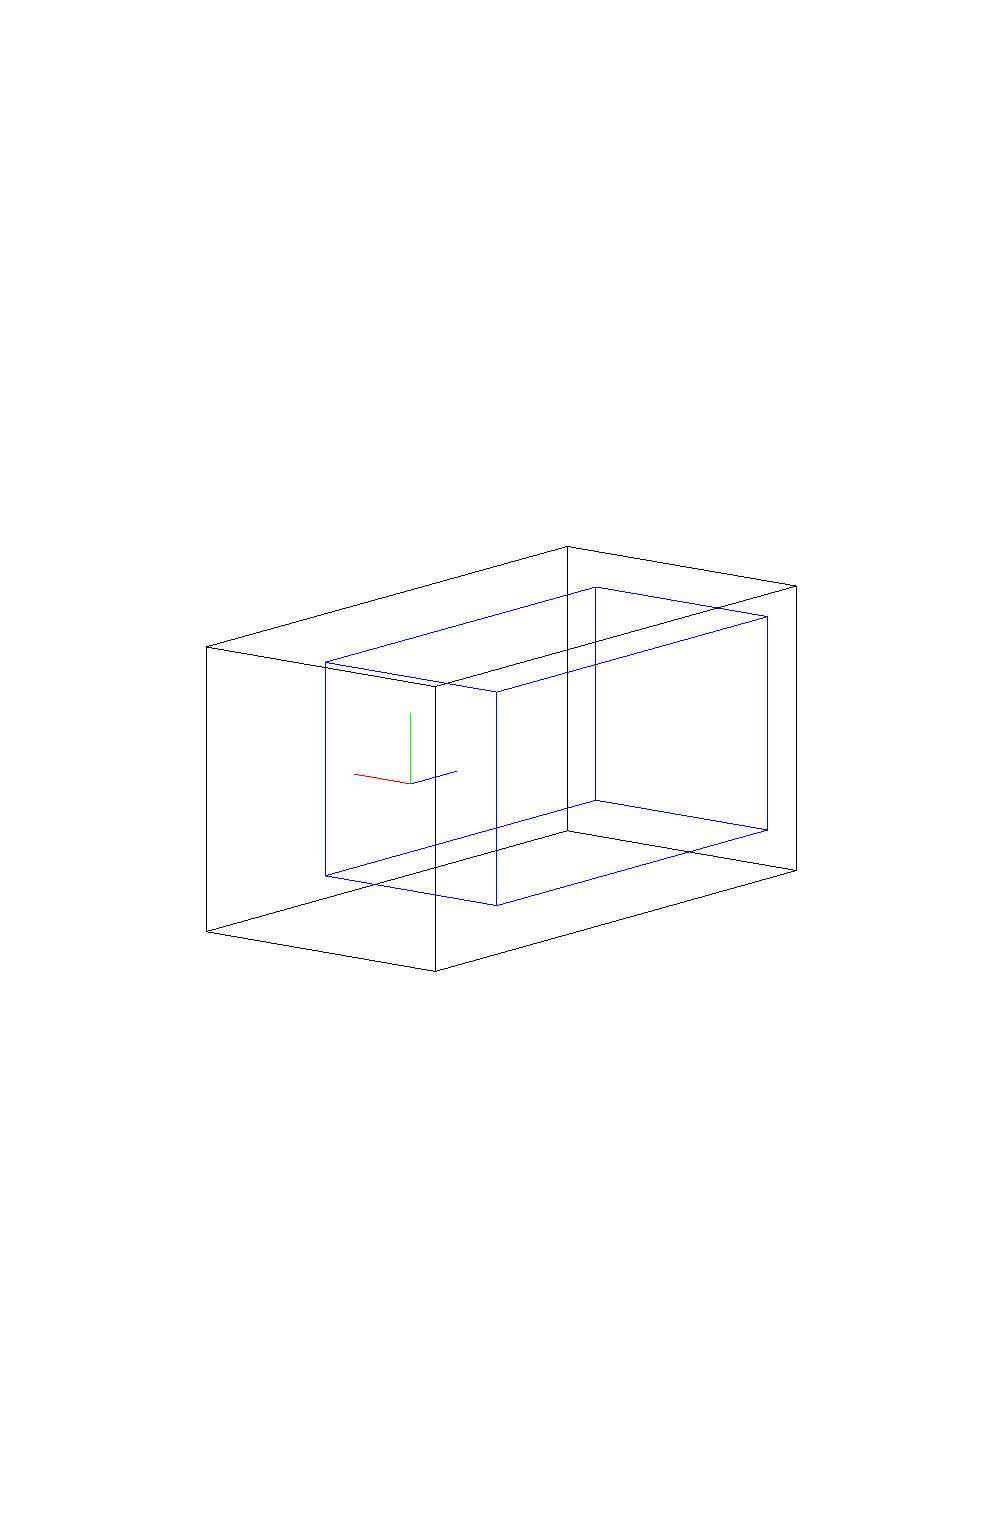
\includegraphics[width=0.5\textwidth]{tex/tiltview.pdf}
\centering\caption{실험실 전체를 비스듬히 본 그림. RGB순으로 $xyz$축이다.}
\end{figure}

\begin{figure}[h]
\centering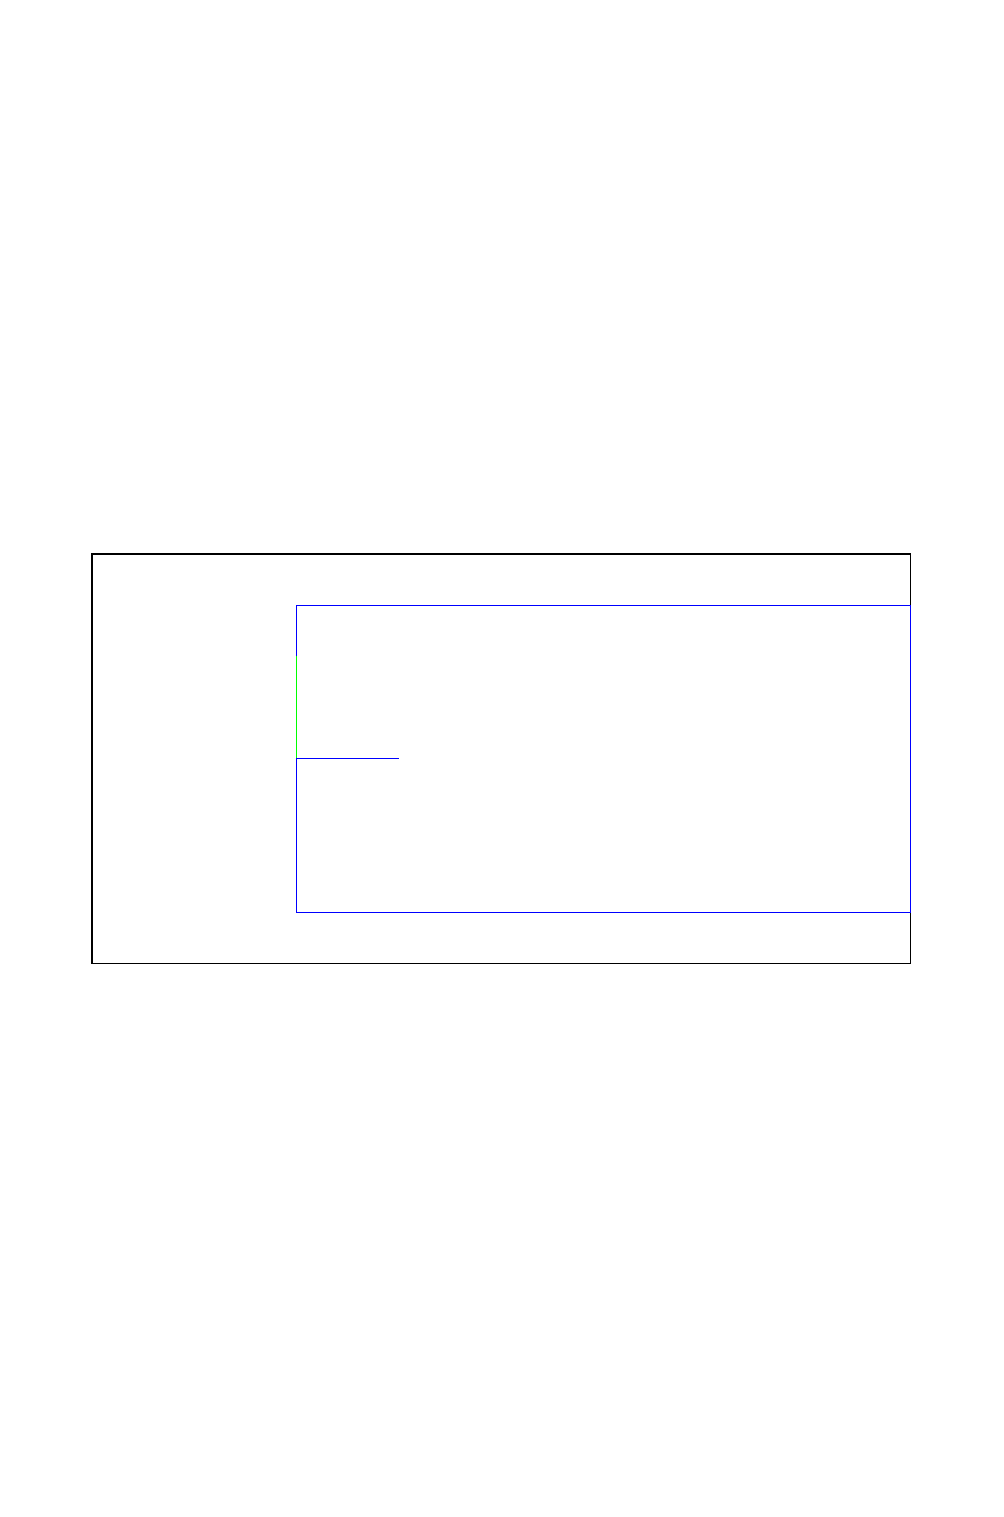
\includegraphics[width=0.5\textwidth]{tex/sideview.pdf}
\centering\caption{실험실 전체를 옆에서 본 그림.}
\end{figure}

실험실 크기는 $20\times20\times40$ cm이고, 검출기로 사용할 Scintillator는
$15\times15\times30$ cm이며, $10\times10\times1$ mm의 작은 조각별로 저장된
에너지를 읽을 수 있다고 가정한다. 이 Scintillator Array의 중심은 $(0, 0, 5
\text{ cm})$에 위치돼 있다. 입사하는 빔은 150 MeV의 양성자 빔을 사용할 것이고,
Scintillator의 바로 앞인 $(0, 0, -10 \text{ cm})$에서 쏠 것이다.

10000개의 양성자를 이러한 구조의 Scintillator에 쏘아서 나온 데이타를 가지고
그래프를 그려보면 그림~\eqref{finalResult}과 같은 결과를 얻을
수 있다.

\begin{figure}[h]
\centering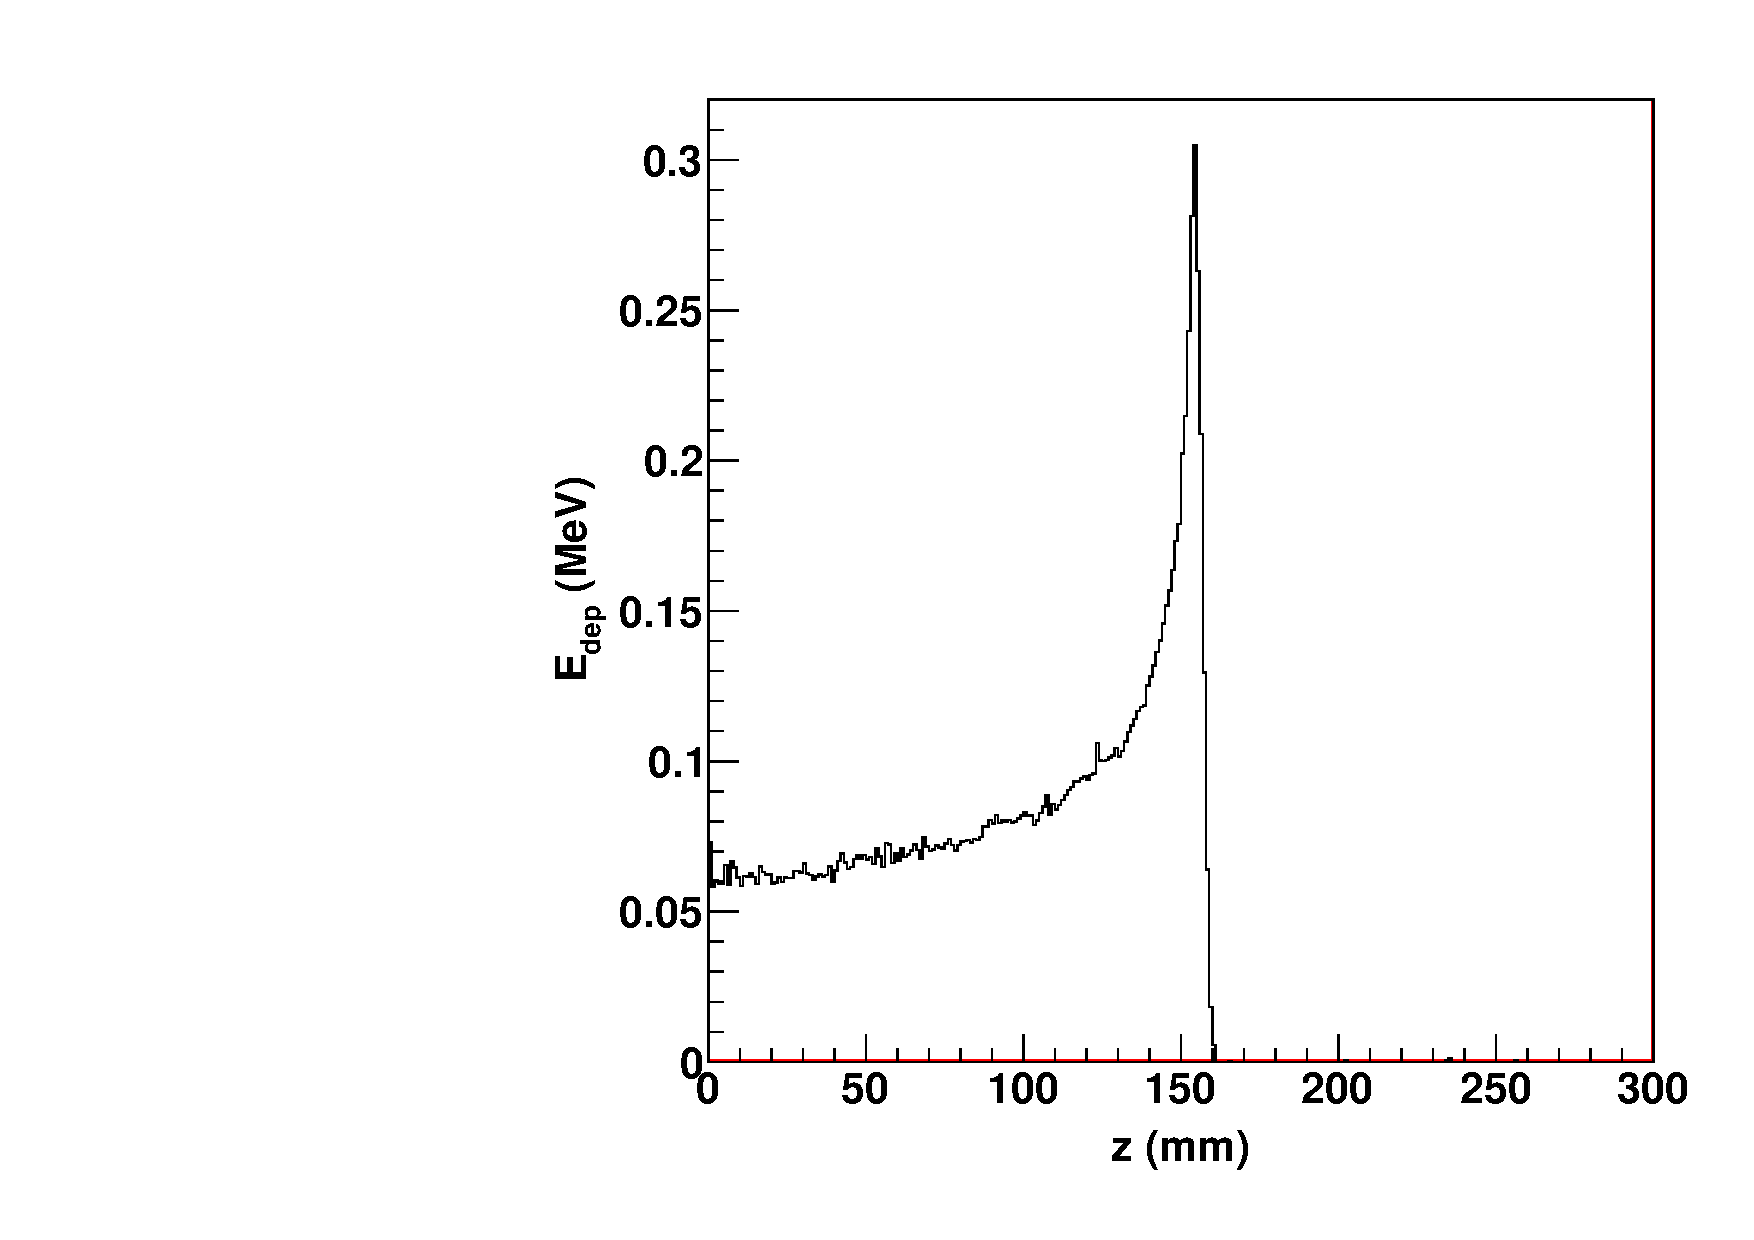
\includegraphics[width=0.7\textwidth]{tex/finalResult.pdf}
\centering\caption{양성자에 의한 Bragg Peak \label{finalResult}}
\end{figure}
